% \title{Case study \#1: Ethical requirements for recomputation}
% \author{
% 	Benjamin M. Gorman \\
%                School of Computing,
%         University of Dundee\\
%         Dundee DD1 4HN, \underline{Scotland}\\
% 	b.gorman@dundee.ac.uk\\
% 	\and\\
% 	Luke Hutton \\
% 		School of Computer Science,
% 		University of St Andrews\\
% 		St Andrews KY16 9SX, \underline{Scotland}\\
% 	lh49@st-andrews.ac.uk	
% 	\and\\
%         Karen Petrie \\
%                School of Computing,
%         	      University of Dundee\\
%         Dundee DD1 4HN, \underline{Scotland}\\
%         kpetrie@dundee.ac.uk 
%        %add yourself here! 
% }
% \date{\today}

% \documentclass[12pt]{article}

% \begin{document}
% \maketitle

\section{Case study \#1: Ethical requirements for recomputation}

\subsection{Introduction}
The goal of recomputation\footnote{http://www.recomputation.org/} is to follow the recompilation manifesto\footnote{http://www.recomputation.org/blog/2013/04/12/the-recomputation-manifesto/} and make computational experiments recomputable by providing tools and a repository to store experiments in. The mission is stated as:
\begin{quote}
``If we can compute your experiment now, anyone can recompute it 20 years from now''
\end{quote}

One of the considerations perhaps under considered in regards to recomputation to date is the ethical implications. 
\subsection{Background}

Due to the nature of an HCI experiment, in that it involves gathering data from human participants, it is necessary in order to successfully replicate an HCI experiment you must gather a new set of participants of which must meet the original experiments inclusion and exclusion criteria. In order for this to occur it is also necessary to replicate the ethical approval which the original experimenter sought, at first this may seem trivial however through examination of ethical approval submissions from ten institutions across the UK, EU, and US we found great differences between each and that a very low amount of overlap currently exists.

\begin{figure}
    \centerline{\resizebox{1\linewidth}{!}{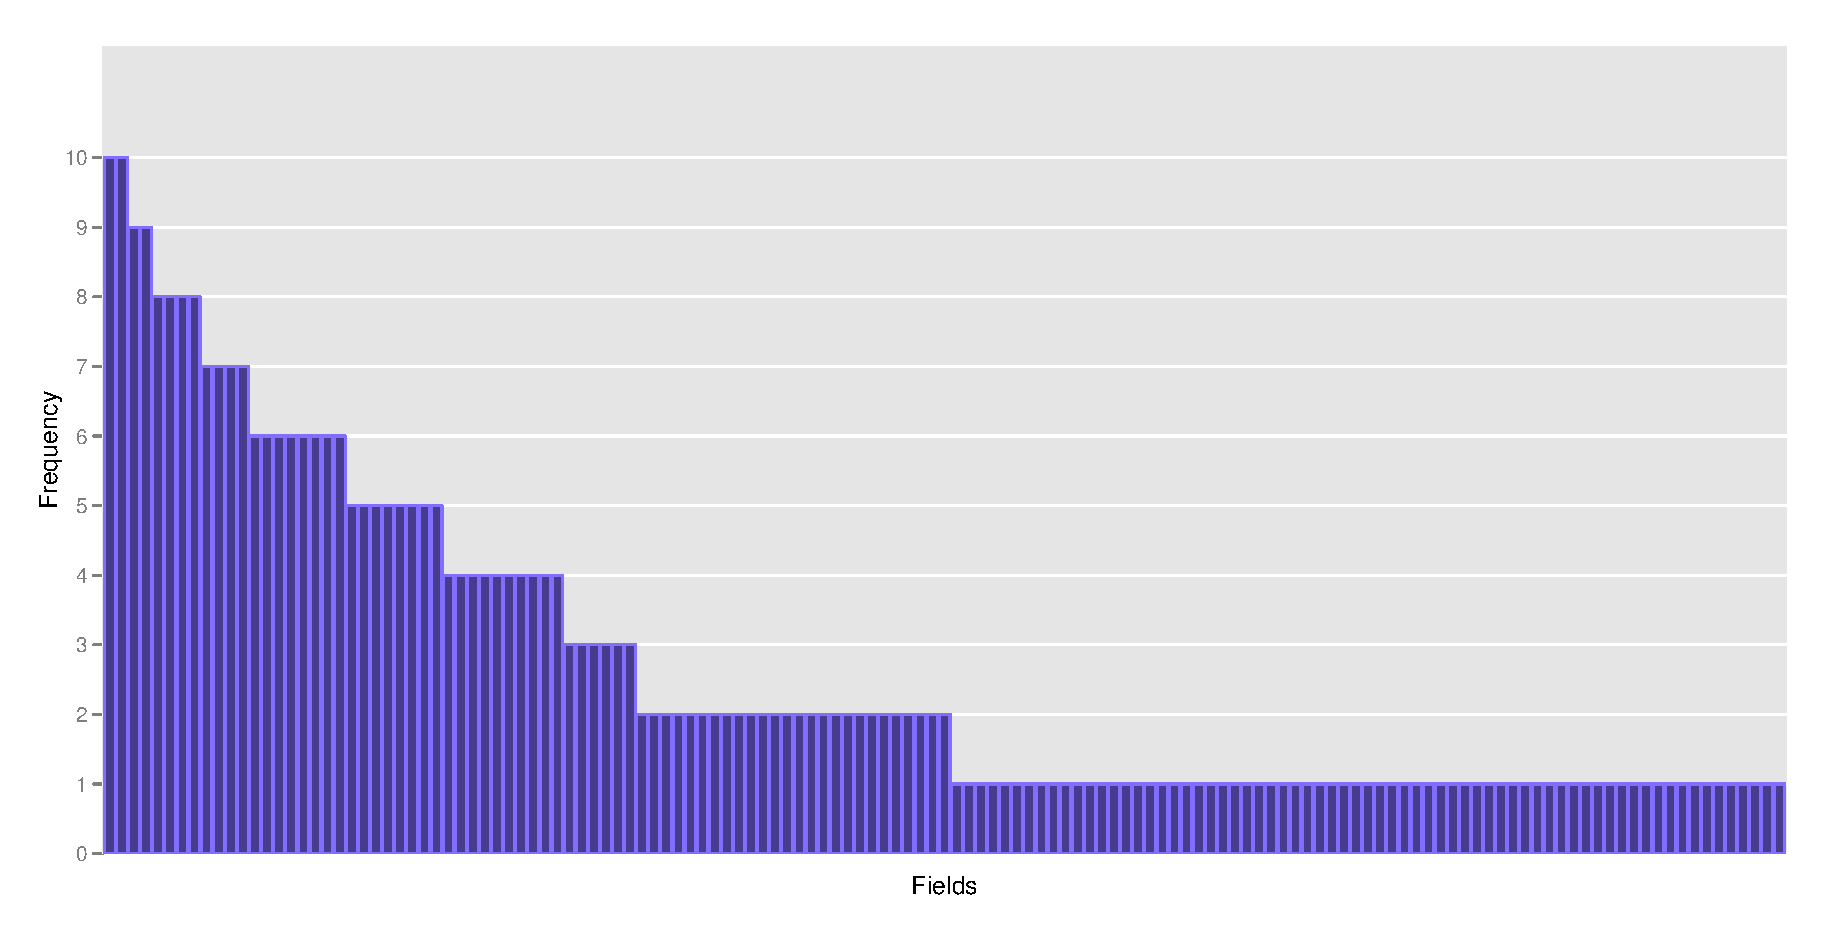
\includegraphics{plot-fieldfreq.eps}}}
    \caption{Histogram showing frequency distribution of fields in ethics applications}
\end{figure}

\subsection{Comparison of Ethical Requirements across Universities}

Through examination of ethics submissions from ten institutions across the UK, EU, and US,
we aim to discover a set of ethical concerns common to all. 
Our analysis uncovered 145 unique fields, 
encompassing generic details, such as contact details of co-investigators, methodological
details, and institution-specific requirements, often for insurance and liability purposes.
Of these fields, only two were common to all ten ethics forms - the name of the principal
investigator, and whether informed consent was sought. While this is clearly insufficient
as a minimum specification for capturing ethics requirements, it reveals the crux of the 
ethics approval process is to ensure participant agency is maintained through the experimental process by mandating informed consent.

Examining the frequency with which these fields occur highlights the 
=======
% Gaterhing forms

Why did we select each institition?

% Comment on openess

% Gathering of unique fields

In order to compare each ethical approval form from each instituion, we manually transcribed each field and noted unique occurances. Minor changes in wording were ignored(?). However, expansions and additional questions were counted as unique fields. Our analysis uncovered 182 unique fields, encompassing generic details, such as contact details of co-investigators, methodological details, and institution-specific requirements, often for insurance and liability purposes. Of these fields, only two were common to all ten ethics forms - the name of the principal investigator, and whether informed consent was sought. While this is clearly an insufficient  minimum specification for capturing ethics requirements, it reveals the crux of the ethics approval process is to ensure participant agency is preserved through the experimental process.





% which fields occur frequently

% thematic overlaps

% surprisingly small common set

% what are the outliers - are they important?


\subsection{Comparison of Ethical Requirements across Publishers}

\subsection{Framework for Ethics to accompany data and experiments}

